% presentation.tex

\documentclass{beamer}
\usetheme{Intel}

% Document configuration
%\setbeameroption{show notes} % If annotations are desired.
\setbeamertemplate{section in toc}{\inserttocsectionnumber.~\inserttocsection} % Use number keys for table of content sections.
\setbeamertemplate{subsection in toc}{\hspace{0.5cm}\rule[0.3ex]{3pt}{3pt}~\inserttocsubsection\par} % Use a symbol for table of content subsections.
\AtBeginSection[]
{
	\begin{frame}
		\frametitle{Table of Contents}
		\begin{multicols}{2}
			\tableofcontents[currentsection]
		\end{multicols}
    \end{frame}
} % Insert table of contents frame before each new section.
\setbeamertemplate{caption}[numbered] % Number figures.

\definecolor{intel}{RGB}{0, 113, 197}
\setbeamercolor{section in toc shaded}{fg=intel}
\setbeamercolor{subsection in toc shaded}{fg=black}
\setbeamercolor{section in toc}{fg=intel}
\setbeamercolor{subsection in toc}{fg=black}
\setbeamercolor{block title}{fg=intel}
\setbeamercolor{caption name}{fg=intel}

% Package inclusion:
\usepackage{tikz} % Used by presentationprogressbar.tex
\usepackage{hyperref} % Used to invoke Santa Claus.
\usepackage{multicol} % Used to split up table of contents in a double column style.
\usepackage{multirow} % Needed for multirow graphs
\usepackage{datetime} % Used to format dates.
\usepackage{pdflscape} % Used to landscape frames.
\usepackage{listings} % Used to format inline code throughout document.
\usepackage{color} % Used to gray out text
\usepackage{tikz} % Used to gain access to the \centering command.

\usepackage[footinfo]{gitinfo} % dv2524-pac/

% Package configuration:
\hypersetup{
	colorlinks=false,
	linkcolor=blue,
	urlcolor=black,
	citecolor=blue,
	anchorcolor=blue
}
\usetikzlibrary{calc}

\newenvironment{graytext}{\color{gray}}{\ignorespacesafterend}

% presentationprogressbar.tex
% Defines a progress bar used at the top of each frame.
% ---
% Written by Gonzalo Medina (http://tex.stackexchange.com/users/3954/gonzalo-medina).
% http://tex.stackexchange.com/questions/59742/progress-bar-for-latex-beamer
% Jun 13 '12
% edited Jun 21 '12

\definecolor{pbblue}{HTML}{0A75A8}% color for the progress bar and the circle 

\makeatletter
\def\progressbar@progressbar{} % the progress bar
\newcount\progressbar@tmpcounta% auxiliary counter
\newcount\progressbar@tmpcountb% auxiliary counter
\newdimen\progressbar@pbht %progressbar height
\newdimen\progressbar@pbwd %progressbar width
\newdimen\progressbar@rcircle % radius for the circle
\newdimen\progressbar@tmpdim % auxiliary dimension

\progressbar@pbwd=\linewidth
\progressbar@pbht=1pt
\progressbar@rcircle=2.5pt

% the progress bar
\def\progressbar@progressbar{%

    \progressbar@tmpcounta=\insertframenumber
    \progressbar@tmpcountb=\inserttotalframenumber
    \progressbar@tmpdim=\progressbar@pbwd
    \multiply\progressbar@tmpdim by \progressbar@tmpcounta
    \divide\progressbar@tmpdim by \progressbar@tmpcountb

  \begin{tikzpicture}
    \draw[pbblue!30,line width=\progressbar@pbht]
      (0pt, 0pt) -- ++ (\progressbar@pbwd,0pt);

    \filldraw[pbblue!30] %
      (\the\dimexpr\progressbar@tmpdim-\progressbar@rcircle\relax, .5\progressbar@pbht) circle (\progressbar@rcircle);

    \node[draw=pbblue!30,text width=3.5em,align=center,inner sep=1pt,
      text=pbblue!70,anchor=east] at (0,0) {\insertframenumber/\inserttotalframenumber};
  \end{tikzpicture}%
}

\addtobeamertemplate{headline}{}
{%
  \begin{beamercolorbox}[wd=\paperwidth,ht=4ex,center,dp=1ex]{white}%
    \progressbar@progressbar%
  \end{beamercolorbox}%
}
\makeatother

% Command to read, and ouput the first line of a file:
\newread\file
\newcommand{\dvtcmdfirstline}[1]{
	\openin\file=#1
	\read\file to \keyval
	\keyval % Return keyval.
	\closein\file
}

\lstset{
	language=C,
	tabsize=4,
	backgroundcolor=\color{black!5},
	basicstyle=\tiny,
}

% Formatting inline code command:
\newcommand{\dvtcmdcodeinline}[1]{
	\colorbox{black!5}{
			\lstinline[basicstyle=\ttfamily\color{black}]{#1}}}

\newtheorem{thm}{Key point}

\begin{document}
	% FRONT MATTER
	% ---
	\title{Paravirtualizing OpenGL ES in Simics}
\subtitle{Master's Thesis in Computer Science}
\author{Eric Nilsson}
\institute{Intel Corporation}
\date{\today}

\begin{frame}
	\titlepage
\end{frame}


	% BODY MATTER
	% ---
	% INTRODUCTION
	\section{Introduction}
	% Simics
	\subsection{Simics}
	\begin{frame}

\frametitle{Wind River\texttrademark\ Simics\texttrademark }

\begin{itemize}
	\item Full-system simulator\note{That is; a fast and functional simulator that runs unmodified software}
	\item Originally devised at SICS\footnote{The Swedish Institute of Computer Science.}\note{This was the first instance of an unmodifed OS running in an entirely simulated environment}
	\item Developed by Intel\textregistered 
	\item Sold through Intels subsidiary Wind River Systems, Inc.
	\item Used in the industry by groups such as:
	\begin{itemize}
		\item IBM
		\item NASA
		\item Lockheed Martin
	\end{itemize}
	\item Utilized extensively in academia\footnote{$300+$ universities.}
\end{itemize}

\end{frame}

	% Graphics virtualization
	\subsection{Graphics virtualization}
	\begin{frame}
\frametitle{Graphics virtualization}

\begin{columns}
	\column{0.5\textwidth}
	\begin{block}{GPU modeling}
		Develop a GPU model virtualizing the GPU Instruction Set Architecture (ISA).
	\end{block}
	\begin{block}{PCI passthrough}
		Utilize passthrough methodology; granting virtual systems first-hand access to host machine devices.
	\end{block}
    \column{0.5\textwidth}
    \begin{block}{Soft modeling}
    	Use advanced software rasterizers optimizing GPU kernel simulation for CPU architectures.
    \end{block}
    \begin{block}{Paravirtualization}
    	Selectively modify the virtual architecture to accomodate scalability, performance, and simplicity.
    \end{block}
\end{columns}
	
\end{frame}

	% Summary
	\subsection{Summary}
	\begin{frame}
  \frametitle{Summary}

  \begin{columns}
  \column{0.5\textwidth}

  \begin{block}{Method}
    \begin{itemize}
    \item Paravirtualized graphics
    \item Accelerates OpenGL ES 2.0
    \end{itemize}
  \end{block}

  \begin{block}{Evaluation}
    \begin{itemize}
    \item Run benchmarks stressing suspected optimal and sub-optimal use-case
    \item Compare performance to software rasterization
    \end{itemize}
  \end{block}

  \begin{block}{Conclusion}
    \begin{itemize}
    \item Improved performance, $34\times$
    \item Located bottleneck
    \end{itemize}
  \end{block}

  \column{0.5\textwidth}

  \begin{center}
    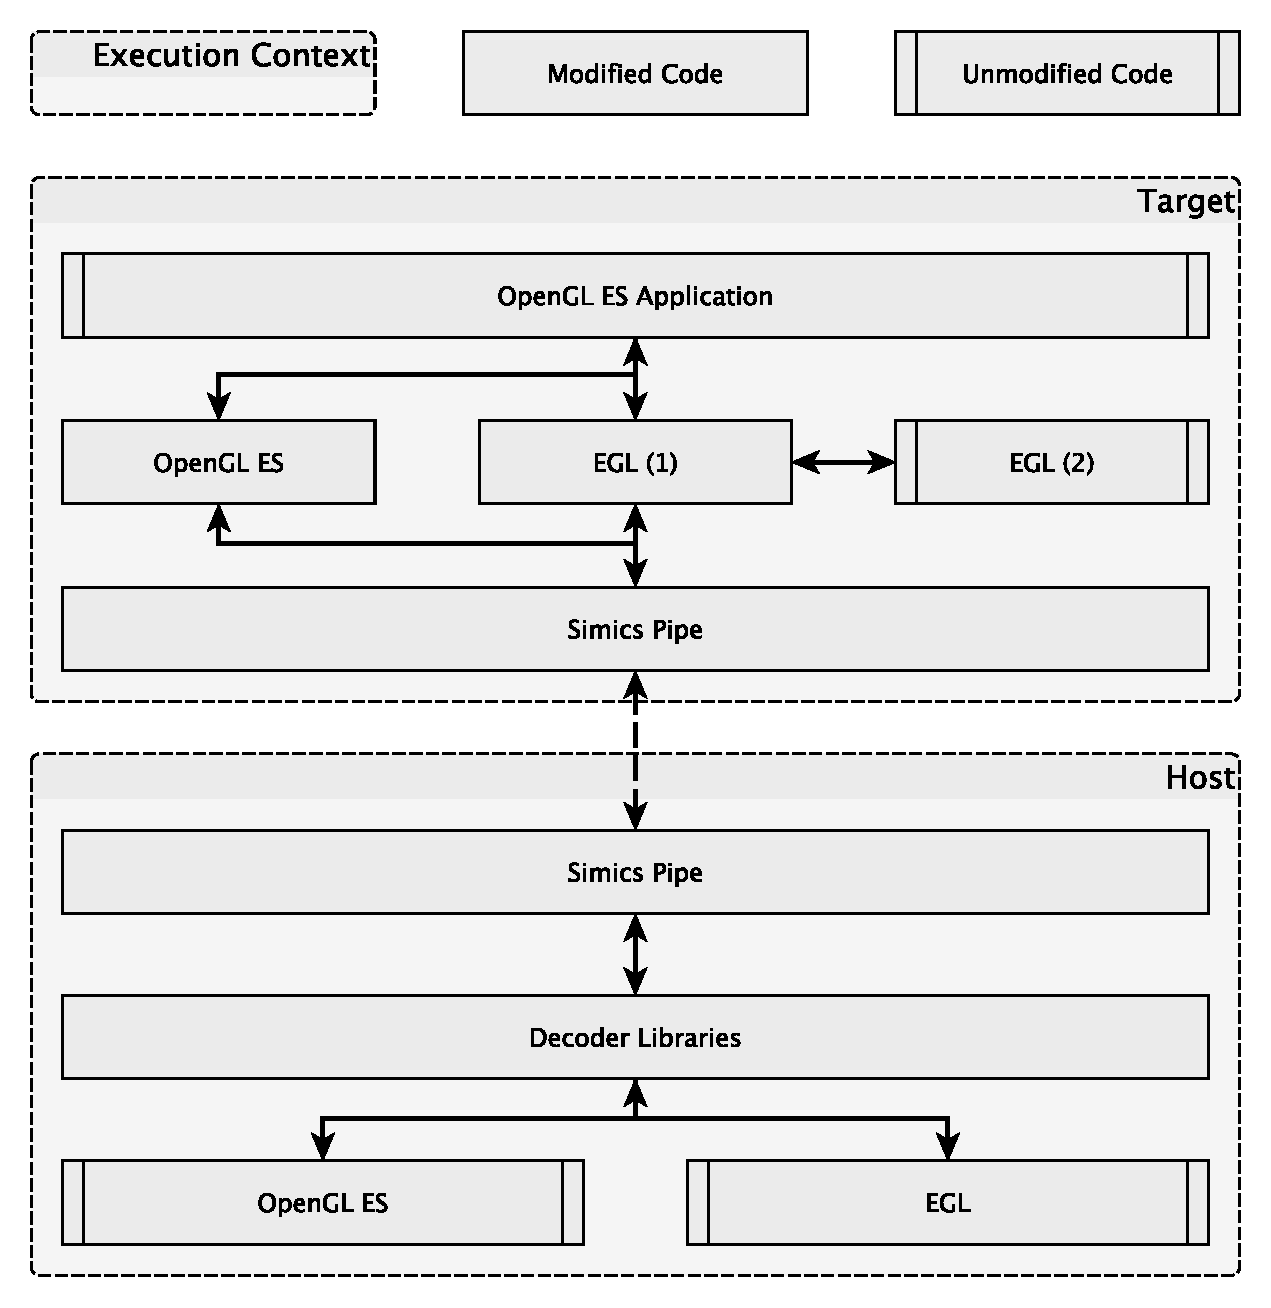
\includegraphics[height=0.7\textheight]{yedoverview.pdf}
  \end{center}

\end{columns}

\end{frame}

	% Key points
	\subsection{Key points}
	\begin{frame}
\frametitle{Question formulation}

\begin{block}{\#1}
  Is paravirtualization is a viable method of accelerating graphics?
\end{block}

\begin{block}{\#2}
  Are magic instructions is a suitable communications medium?
\end{block}

\begin{block}{\#3}
  How does hardware-assisted virtualization impact graphics acceleration using paravirtualization?
\end{block}

\end{frame}


	% PARAVIRTUALIZATION
	\section{Methodology}
	% Overview
	\subsection{Overview}
	% presentationoverview.tex

\begin{frame}
\frametitle{Overview}

\begin{center}
	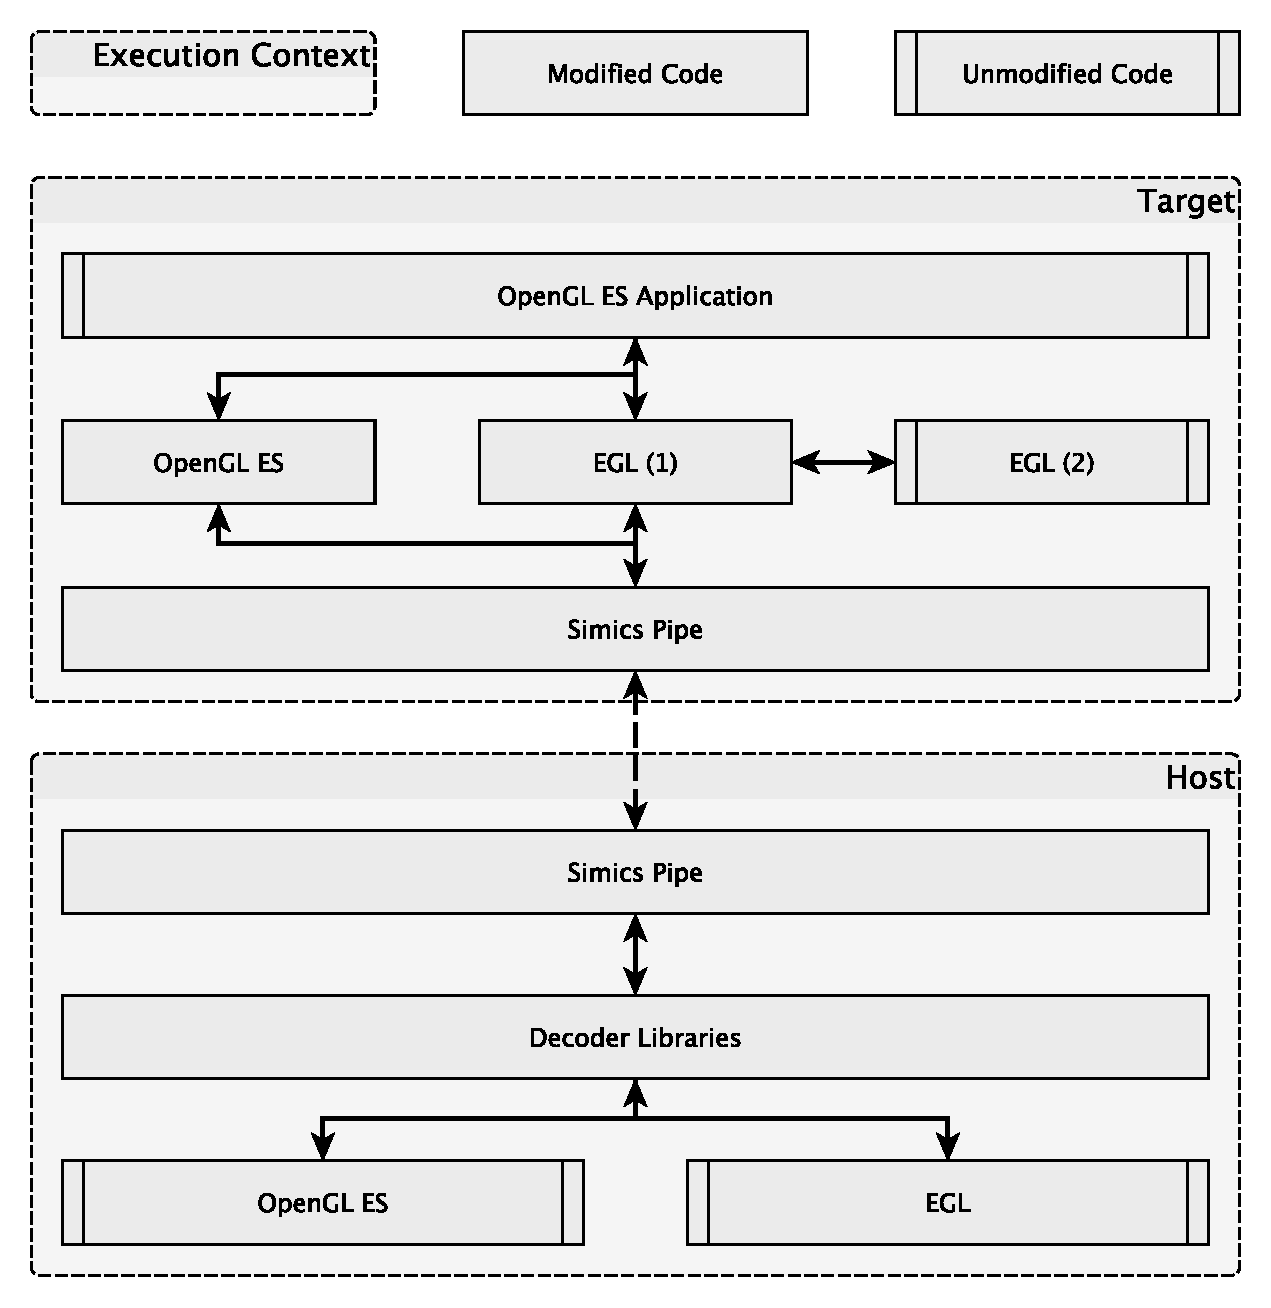
\includegraphics[height=0.8\textheight]{yedoverview.pdf}
\end{center}

\end{frame}

	% Magic instructions
	\subsection{Magic instructions}
	\begin{frame}
\frametitle{Magic instructions}

\begin{block}{Background}
	\begin{itemize}
		\item Many resons to escape simulation
		\begin{itemize}
			\item Breakpoints
			\item File sharing
			\item Profiling
		\end{itemize}
		\item Several methodologies
	\end{itemize}
\end{block}

\begin{block}{The 'Magic instruction'}
	\begin{itemize}
		\item \dvtcmdcodeinline{nop}-type instruction\footnotemark
		\item Potentially instant
		\item No modification to target system
	\end{itemize}
\end{block}

\footnotetext{\dvtcmdcodeinline{xchg ebx, ebx}}

\end{frame}

	% Simics Pipe
	\subsection{Simics Pipe}
	\begin{frame}
\frametitle{Simics Pipe}

\begin{center}
	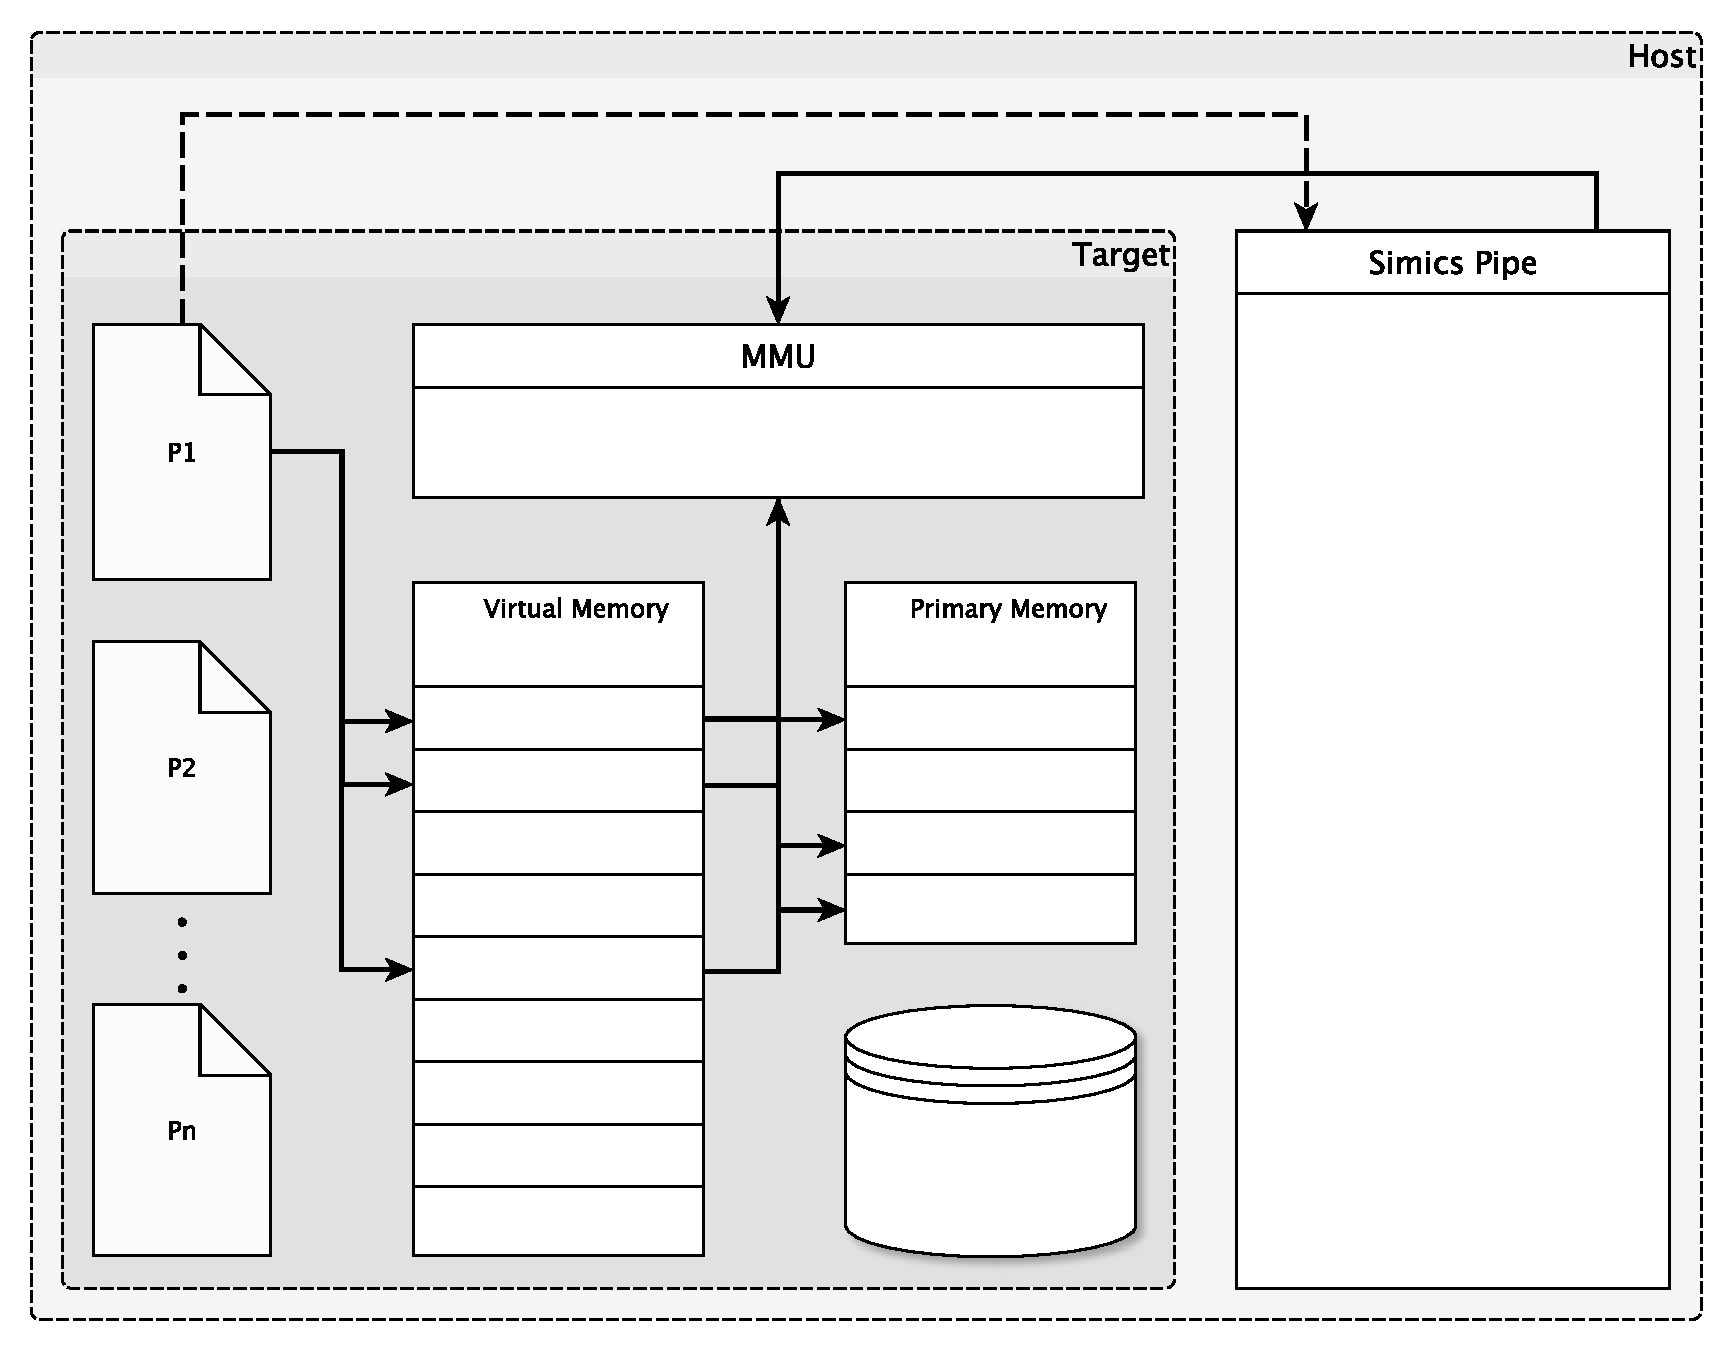
\includegraphics[height=0.8\textheight]{yedvirtualmemory.pdf}
\end{center}

\end{frame}

%% Memory translation overview. The OpenGL process hands a virtual memory
%% address, pointing somewhere in the target system \textit{primary}
%% memory, to the paravirtualized solution - which inquiries the target
%% system MMU to retrieve designated bytestream directly from target
%% physical memory.


	% EXPERIMENT
	\section{Experiment}
	% Benchmarks
	\subsection{Benchmarks}
	\begin{frame}[allowframebreaks]
\frametitle{Benchmarks}

%% % figbenchmarks.tex

\begin{figure}

\minipage{0.32\textwidth}
	
\includegraphics[width=\linewidth]{imgchess.png}
	\caption[Chess benchmark screen capture]{Chess.}
	\label{fig:benchmarks_chess}
\endminipage\hfill
\minipage{0.32\textwidth}
	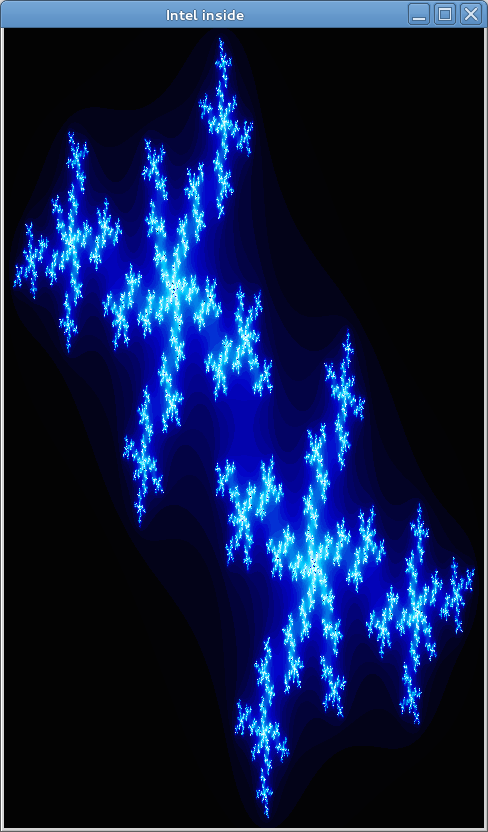
\includegraphics[width=\linewidth]{imgjulia.png}
	\caption[Julia benchmark screen capture]{Julia.}
	\label{fig:benchmarks_julia}
\endminipage\hfill
\minipage{0.32\textwidth}
  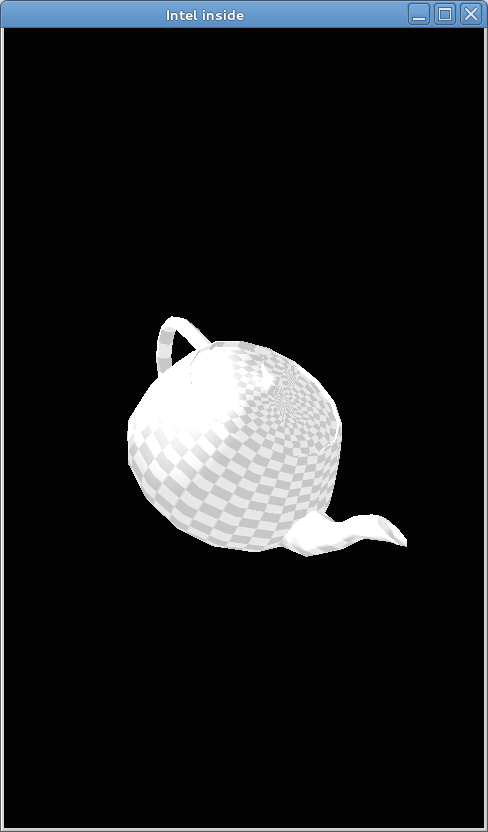
\includegraphics[width=\linewidth]{imgphong.png}
  \caption[Phong benchmark screen capture]{Phong.}
  \label{fig:benchmarks_phong}
\endminipage

\end{figure}

\framebreak 

%% \begin{block}{Input data variation}
%% \center
%% \resizebox{\linewidth}{!}{%
%% 	% tabkeyvals.tex

\begin{tabular}{lllll}
	Benchmark	& Input Data			& Halved Input		& Ref. Input		& Double Input		\\ \hline
	Chess		& No. Tiles				& $60\times60$		& $84\times84$		& $118\times118$	\\
	Julia		& No. Iterations		& $225$				& $450$				& $900$				\\
	Phong		& Texture Resolution	& $1448\times1448$	& $2048\times2048$	& $2896\times2896$	\\
\end{tabular}

%% }
%% \end{block}

%% \begin{block}{No. magic instructions}
%% \center
%% \resizebox{\linewidth}{!}{%
%% 	% tabkeyvalsmagicinstructions.tex

\begin{tabular}{lllll}
	Benchmark	& \phantom{Input Data}			& Halved Input	& Ref. Input	& Double Input	\\ \hline
	Chess		& \phantom{No. Tiles}			& $32403$		& $63507$		& $125319$		\\
	Julia		& \phantom{No. Iterations}		& $16$			& $16$			& $16$			\\
	Phong		& \phantom{Texture Resolution}	& $17$ 			& $17$ 			& $17$		\\
\end{tabular}

%% }
%% \end{block}
	
\end{frame}


	% RESULTS
	\section{Results}
	% Results - Host
	\subsection{Reference histograms}
	% presentationresultshost.tex

\begin{frame}
\frametitle{Host and QEMU histograms}

%% \begin{columns}
%% 	\column{0.5\textwidth}
%% 	\centering
%% 	% histogramshost
%% 	\resizebox*{!}{0.8\textheight}{%
%% 		\input{gnuhistogramshost.tex}
%% 	}
%%     \column{0.5\textwidth}
%%     \centering
%%     % histogramsqemu
%% 	\resizebox*{!}{0.8\textheight}{%
%% 		\input{gnuhistogramsqemu.tex}
%% 	}
%% \end{columns}
	
\end{frame}

	% Results - Chess
	\subsection{Chess histograms}
	\begin{frame}
  \frametitle{Results - Chess}

  \begin{table}[]
    \centering
    \begin{tabular}{lllll}
      \hline
      Input & \multicolumn{4}{l}{Elapsed time (ms)} \\ \hline
      Tiles & Min & Max & Std & Avg \\
      $60\times60$ & \mascfirstline{simicschess60x60.dat.min} & \mascfirstline{simicschess60x60.dat.max} & \mascfirstline{simicschess60x60.dat.std} & \textbf{\mascfirstline{simicschess60x60.dat.avg}} \\
      $84\times84$ & \mascfirstline{simicschess84x84.dat.min} & \mascfirstline{simicschess84x84.dat.max} & \mascfirstline{simicschess84x84.dat.std} & \textbf{\mascfirstline{simicschess84x84.dat.avg}} \\
      $118\times118$ & \mascfirstline{simicschess118x118.dat.min} & \mascfirstline{simicschess118x118.dat.max} & \mascfirstline{simicschess118x118.dat.std} & \textbf{\mascfirstline{simicschess118x118.dat.avg}} \\ \hline
    \end{tabular}
    \caption{Software rasterization}
  \end{table}

  \begin{table}[]
    \centering
    \begin{tabular}{lllll}
      \hline
      Input & \multicolumn{4}{l}{Elapsed time (ms)} \\ \hline
      Tiles & Min & Max & Std & Avg \\
      $60\times60$ & \mascfirstline{parachess60x60.dat.min} & \mascfirstline{parachess60x60.dat.max} & \mascfirstline{parachess60x60.dat.std} & \textbf{\mascfirstline{parachess60x60.dat.avg}} \\
      $84\times84$ & \mascfirstline{parachess84x84.dat.min} & \mascfirstline{parachess84x84.dat.max} & \mascfirstline{parachess84x84.dat.std} & \textbf{\mascfirstline{parachess84x84.dat.avg}} \\
      $118\times118$ & \mascfirstline{parachess118x118.dat.min} & \mascfirstline{parachess118x118.dat.max} & \mascfirstline{parachess118x118.dat.std} & \textbf{\mascfirstline{parachess118x118.dat.avg}} \\ \hline
    \end{tabular}
    \caption{Paravirtualization}
  \end{table}

\end{frame}

    %% \begin{table}
    %%   \resizebox{0.95\columnwidth}{!}{%
    %%   \begin{tabular}{|c|c|r|r|r|r|}
    %%     \hline
    %%     \multirow{2}{*}{Benchmark} & \multirow{2}{*}{Input} & \multicolumn{4}{p{4cm}|}{\centering Elapsed time (\milli\second )} \\
    %%     \cline{3-6} && \multicolumn{1}{c|}{Min} & \multicolumn{1}{c|}{Max} & \multicolumn{1}{c|}{Std} & \multicolumn{1}{c|}{Avg} \\ \hline
    %%     \multirow{3}{*}{Chess} & \chesskeyone & \mascfirstline{parachess60x60.dat.min} & \mascfirstline{parachess60x60.dat.max} & \mascfirstline{parachess60x60.dat.std} & \textbf{\mascfirstline{parachess60x60.dat.avg}} \\
    %%     & \chesskeytwo & \mascfirstline{parachess84x84.dat.min} & \mascfirstline{parachess84x84.dat.max} & \mascfirstline{parachess84x84.dat.std} & \textbf{\mascfirstline{parachess84x84.dat.avg}} \\
    %%     & \chesskeythree & \mascfirstline{parachess118x118.dat.min} & \mascfirstline{parachess118x118.dat.max} & \mascfirstline{parachess118x118.dat.std} & \textbf{\mascfirstline{parachess118x118.dat.avg}} \\ \hline
    %%     \multirow{3}{*}{Julia} & \juliakeyone & \mascfirstline{parajulia225.dat.min} & \mascfirstline{parajulia225.dat.max}	& \mascfirstline{parajulia225.dat.std} & \textbf{\mascfirstline{parajulia225.dat.avg}} \\
    %%     & \juliakeytwo & \mascfirstline{parajulia450.dat.min} & \mascfirstline{parajulia450.dat.max} & \mascfirstline{parajulia450.dat.std} & \textbf{\mascfirstline{parajulia450.dat.avg}} \\
    %%     & \juliakeythree & \mascfirstline{parajulia900.dat.min} & \mascfirstline{parajulia900.dat.max} & \mascfirstline{parajulia900.dat.std} & \textbf{\mascfirstline{parajulia900.dat.avg}} \\ \hline
    %%   \end{tabular}
    %%   }
    %%   \caption{Paravirtualization}
    %% \end{table}

	% Results - Julia
	\subsection{Julia histograms}
	% presentationresultsjulia.tex

\begin{frame}
\frametitle{Simics histograms: Julia}

\begin{center}
\resizebox{0.8\textwidth}{!}{%
	\input{gnuhistogramssimicsparajulia.tex}
}
\end{center}

\end{frame}
	% Results - Phong
	\subsection{Phong histograms}
	% presentationresultsphong.tex

\begin{frame}
\frametitle{Simics histograms: Phong}

%% \begin{center}
%% \resizebox{0.8\textwidth}{!}{%
%% 	\input{gnuhistogramssimicsparaphong.tex}
%% }
%% \end{center}

\end{frame}

	% Magic instruction overhead
	\subsection{Magic instruction overhead}
	% presentationmagicinstructionoverhead.tex

\begin{frame}[fragile]
\frametitle{Magic instruction overhead}
%% \begin{figure}
%% \centering
%% \begin{lstlisting}
%% int sercon = open("/dev/ttyS0",O_RDWR|O_NOCTTY);
%% \end{lstlisting}
%% \begin{minipage}{.5\textwidth}
%% 	\centering
	
%% \lstinputlisting{pseudoindividual.txt}
%% \end{minipage}%
%% \begin{minipage}{.5\textwidth}
%% 	\centering

%% \lstinputlisting{pseudobatch.txt}
%% \end{minipage}
%% \end{figure}

%% \begin{center}
%% % tabmagicinstructionsforall.tex

\begin{tabular}{llll}
Min & Max & Std & Avg \\ \hline
\dvtcmdfirstline{magicinstrprofileall.dat.min} & \dvtcmdfirstline{magicinstrprofileall.dat.max} & \dvtcmdfirstline{magicinstrprofileall.dat.std} & \dvtcmdfirstline{magicinstrprofileall.dat.avg} \\
\end{tabular}

%% \end{center}

\end{frame}


	% DISCUSSION
	\section{Discussion}
	% Deterministic execution
	\subsection{Deterministic execution}
	\begin{frame}

\frametitle{Deterministic execution}

Host dependency may affect simulation determinism\footnote{Variance affects only cross-platform simulation (checkpoints)}:
\begin{itemize}
	\item Hardware GPU floating point accuracy\footnote{Less of an issue since commonplace double floating point precision (2007)}
	\item Software API conformance (specification not necessarily strict)
\end{itemize}

However:
\begin{itemize}
	\item Often not an issue since graphics are commonly used only to display data
	\item Yet, GPU utilization for general purpose workloads increasingly more common
\end{itemize}

\textbf{Example}

\end{frame}

	% Checkpointing
	\subsection{Checkpointing}
	\begin{frame}

\frametitle{Checkpointing}

\begin{block}{Conditions}
	\begin{itemize}
		\item Requires efficient framework functionality to store and restore system states (contestant:\dvtcmdcodeinline{glGet})
		\item Volatility; probable to be platform dependant in terms of efficiency
	\end{itemize}
\end{block}

\begin{block}{Related Work}
	Has been implemented in QEMU for OpenGL (Lagar-Cavilla et al.)
\end{block}

\begin{block}{Future Work}
	\begin{itemize}
		\item Transaction transparency in modern frameworks may advance the Checkpoint/Restart scheme in virtual platforms
		\item Experimental checkpoint schemes have been developed for CUDA (Guo et al.)
	\end{itemize}
\end{block}

\end{frame}

	% Reverse execution
	\subsection{Reverse execution}
	\begin{frame}

\frametitle{Reverse execution}

\begin{block}{Currently}
	Graphics displayed exclusively in the host system
\end{block}

\begin{block}{Assumption}
	A potential productification of paravirtualized graphics would feature graphics output in the target system
\end{block}

\begin{block}{Prediction}
	\begin{itemize}
		\item If so, framebuffers would be present in target memory
		\item It follows that reverse execution functionality in Simics tracks said memory in checkpoints; effectively accomodating for reverse execution graphics
	\end{itemize}
\end{block}

\end{frame}


	% CONCLUSION
	\section{Conclusion}
	% Demonstration
	\subsection{Demonstration}
	\begin{frame}	

\frametitle{Demonstration}

\begin{block}{Julia Benchmark}
	\begin{itemize}
		\item \href{http://youtube.com/embed/GKs6OlWKFV8?rel=0&vq=hd1080&autoplay=1}{[Hardware accelerated on the simulation host]}
		\item \href{http://youtube.com/embed/3sCyzppFL0w?rel=0&vq=hd1080&autoplay=1}{[Software rasterized on the simulation target]}
		\item \href{http://youtube.com/embed/__d_EeZBzwc?rel=0&vq=hd1080&autoplay=1}{[Paravirtualized on the simulation target]}
	\end{itemize}
\end{block}

\end{frame}

	% Future work
	\subsection{Future work}
	\begin{frame}

\frametitle{Future work}

\begin{itemize}
  \item Command serialization batching \begin{itemize}\item WireGL\end{itemize}
  \item Extending supported frameworks \begin{itemize}\item DirectX $\rightarrow$ OpenGL\end{itemize}
  \item General purpose, GPGPU \begin{itemize}\item OpenCL\end{itemize}
\end{itemize}

\end{frame}

	% Key point recap
	\subsection{Key points recap}
	\begin{frame}
\frametitle{Question formulation}

\begin{block}{\#1}
  Is paravirtualization is a viable method of accelerating graphics?
\end{block}

\begin{block}{\#2}
  Are magic instructions is a suitable communications medium?
\end{block}

\begin{block}{\#3}
  How does hardware-assisted virtualization impact graphics acceleration using paravirtualization?
\end{block}

\end{frame}


	% BACK MATTER
	% ---
	% Colophon
	% presentationcolophon.tex

% TODO:
% Add colophon acknowledging progress bar.

\begin{frame}[t]

\frametitle{Colophon}

\begin{tabular}{p{\textwidth}}
{\tiny This presentation is typeset in the Beamer class by Till Tantau using the \LaTeX\ typesetting system by Leslie Lamport, originally devised from Donald Knuth's \TeX .
The progress bar at the top of each frame is authored by Gonzalo Medina.
Furthermore, the environment utilizes packages by Brent Longborough to extract Git metadata.
Graphs are compiled using GNUplot and figures have been devised using yEd.
The document is revision controlled using Git and hosted on GitHub; whilst being built using Python.}
\end{tabular}

\begin{tabular}{p{\textwidth}}
{\tiny Intel and the Intel logo are trademarks of Intel Corporation in the U.S. and/or other countries.
All other trademarks are the property of their respective owners.}
\end{tabular}

\end{frame}


	% Back page
	% presentationback.tex

\newcommand{\commitlink}{https://github.com/CaterHatterPillar/dv2524/commit/}
\expandafter\def\expandafter\commitlink\expandafter{\commitlink \gitAbbrevHash}

\yyyymmdddate
\renewcommand{\dateseparator}{-} % To print date in same format as gitinfo-package.

\begin{frame}[t]

{\tiny This document was compiled \today\ and last edited by \gitAuthorName\ \gitAuthorDate .\\
The revision may be identified by commit hash \href{\commitlink}{\texttt{\gitAbbrevHash}}}.

\end{frame}

	% Tables
	\begin{landscape}
\begin{frame}
\frametitle{}
\begin{center}

Software rasterized:
% keyvalsimics
%% \resizebox{\linewidth}{!}{%
%% 	% tabkeyvalsimics.tex

% This ought be made into an environment.

\providecommand{\chesskeyone}{$60\times60$ tiles}
\providecommand{\chesskeytwo}{$84\times84$ tiles}
\providecommand{\chesskeythree}{$118\times118$ tiles}

\providecommand{\juliakeyone}{$225$ iterations}
\providecommand{\juliakeytwo}{$450$ iterations}
\providecommand{\juliakeythree}{$900$ iterations}

\providecommand{\phongkeyone}{$1448\times1448$ texels}
\providecommand{\phongkeytwo}{$2048\times2048$ texels}
\providecommand{\phongkeythree}{$2896\times2896$ texels}

\begin{tabular}{|c|c|c|c|c|c|}
\hline
\multirow{2}{*}{Benchmark} & \multirow{2}{*}{Key} & \multicolumn{4}{p{6cm}|}{\centering Elapsed time (milliseconds)} \\
\cline{3-6} && \multicolumn{1}{c|}{Min} & \multicolumn{1}{c|}{Max} & \multicolumn{1}{c|}{Std} & \multicolumn{1}{c|}{Avg} \\ \hline
\multirow{3}{*}{Chess} & \chesskeyone & \dvtcmdfirstline{simicschess60x60.dat.min}		& \dvtcmdfirstline{simicschess60x60.dat.max}		& \dvtcmdfirstline{simicschess60x60.dat.std}		& \dvtcmdfirstline{simicschess60x60.dat.avg} \\ %\cline{2-6}
& \chesskeytwo & \dvtcmdfirstline{simicschess84x84.dat.min} & \dvtcmdfirstline{simicschess84x84.dat.max} & \dvtcmdfirstline{simicschess84x84.dat.std} & \dvtcmdfirstline{simicschess84x84.dat.avg} \\ %\cline{2-6}
& \chesskeythree & \dvtcmdfirstline{simicschess118x118.dat.min} & \dvtcmdfirstline{simicschess118x118.dat.max} & \dvtcmdfirstline{simicschess118x118.dat.std} & \dvtcmdfirstline{simicschess118x118.dat.avg} \\ \hline
\multirow{3}{*}{Julia} & \juliakeyone & \dvtcmdfirstline{simicsjulia225.dat.min}		& \dvtcmdfirstline{simicsjulia225.dat.max}		& \dvtcmdfirstline{simicsjulia225.dat.std} & \dvtcmdfirstline{simicsjulia225.dat.avg} \\ %\cline{2-6}
& \juliakeytwo & \dvtcmdfirstline{simicsjulia450.dat.min} & \dvtcmdfirstline{simicsjulia450.dat.max} & \dvtcmdfirstline{simicsjulia450.dat.std} & \dvtcmdfirstline{simicsjulia450.dat.avg} \\ %\cline{2-6}
& \juliakeythree & \dvtcmdfirstline{simicsjulia900.dat.min} & \dvtcmdfirstline{simicsjulia900.dat.max} & \dvtcmdfirstline{simicsjulia900.dat.std} & \dvtcmdfirstline{simicsjulia900.dat.avg} \\ \hline
\multirow{3}{*}{Phong} & \phongkeyone & \dvtcmdfirstline{simicsphong1448x1448.dat.min}		& \dvtcmdfirstline{simicsphong1448x1448.dat.max}		& \dvtcmdfirstline{simicsphong1448x1448.dat.std}		& \dvtcmdfirstline{simicsphong1448x1448.dat.avg} \\ %\cline{2-6}
& \phongkeytwo & \dvtcmdfirstline{simicsphong2048x2048.dat.min} & \dvtcmdfirstline{simicsphong2048x2048.dat.max} & \dvtcmdfirstline{simicsphong2048x2048.dat.std} & \dvtcmdfirstline{simicsphong2048x2048.dat.avg} \\ %\cline{2-6}
& \phongkeythree & \dvtcmdfirstline{simicsphong2896x2896.dat.min} & \dvtcmdfirstline{simicsphong2896x2896.dat.max} & \dvtcmdfirstline{simicsphong2896x2896.dat.std} & \dvtcmdfirstline{simicsphong2896x2896.dat.avg} \\ \hline
\end{tabular}

%% }

\vspace{1cm}

Paravirtualized:
% keyvalpara
%% \resizebox{\linewidth}{!}{%
%% 	% tabkeyvalpara.tex

% This ought be made into an environment.

\providecommand{\chesskeyone}{$60\times60$ tiles}
\providecommand{\chesskeytwo}{$84\times84$ tiles}
\providecommand{\chesskeythree}{$118\times118$ tiles}

\providecommand{\juliakeyone}{$225$ iterations}
\providecommand{\juliakeytwo}{$450$ iterations}
\providecommand{\juliakeythree}{$900$ iterations}

\providecommand{\phongkeyone}{$1448\times1448$ texels}
\providecommand{\phongkeytwo}{$2048\times2048$ texels}
\providecommand{\phongkeythree}{$2896\times2896$ texels}

\begin{tabular}{|c|c|c|c|c|c|}
\hline
\multirow{2}{*}{Benchmark} & \multirow{2}{*}{Key} & \multicolumn{4}{p{6cm}|}{\centering Elapsed time (milliseconds)} \\
\cline{3-6} && \multicolumn{1}{c|}{Min} & \multicolumn{1}{c|}{Max} & \multicolumn{1}{c|}{Std} & \multicolumn{1}{c|}{Avg} \\ \hline
\multirow{3}{*}{Chess} & \chesskeyone & \dvtcmdfirstline{parachess60x60.dat.min}		& \dvtcmdfirstline{parachess60x60.dat.max}		& \dvtcmdfirstline{parachess60x60.dat.std}		& \dvtcmdfirstline{parachess60x60.dat.avg} \\ %\cline{2-6}
& \chesskeytwo & \dvtcmdfirstline{parachess84x84.dat.min} & \dvtcmdfirstline{parachess84x84.dat.max} & \dvtcmdfirstline{parachess84x84.dat.std} & \dvtcmdfirstline{parachess84x84.dat.avg} \\ %\cline{2-6}
& \chesskeythree & \dvtcmdfirstline{parachess118x118.dat.min} & \dvtcmdfirstline{parachess118x118.dat.max} & \dvtcmdfirstline{parachess118x118.dat.std} & \dvtcmdfirstline{parachess118x118.dat.avg} \\ \hline
\multirow{3}{*}{Julia} & \juliakeyone & \dvtcmdfirstline{parajulia225.dat.min}		& \dvtcmdfirstline{parajulia225.dat.max}		& \dvtcmdfirstline{parajulia225.dat.std} & \dvtcmdfirstline{parajulia225.dat.avg} \\ %\cline{2-6}
& \juliakeytwo & \dvtcmdfirstline{parajulia450.dat.min} & \dvtcmdfirstline{parajulia450.dat.max} & \dvtcmdfirstline{parajulia450.dat.std} & \dvtcmdfirstline{parajulia450.dat.avg} \\ %\cline{2-6}
& \juliakeythree & \dvtcmdfirstline{parajulia900.dat.min} & \dvtcmdfirstline{parajulia900.dat.max} & \dvtcmdfirstline{parajulia900.dat.std} & \dvtcmdfirstline{parajulia900.dat.avg} \\ \hline
\multirow{3}{*}{Phong} & \phongkeyone & \dvtcmdfirstline{paraphong1448x1448.dat.min}		& \dvtcmdfirstline{paraphong1448x1448.dat.max}		& \dvtcmdfirstline{paraphong1448x1448.dat.std}		& \dvtcmdfirstline{paraphong1448x1448.dat.avg} \\ %\cline{2-6}
& \phongkeytwo & \dvtcmdfirstline{paraphong2048x2048.dat.min} & \dvtcmdfirstline{paraphong2048x2048.dat.max} & \dvtcmdfirstline{paraphong2048x2048.dat.std} & \dvtcmdfirstline{paraphong2048x2048.dat.avg} \\ %\cline{2-6}
& \phongkeythree & \dvtcmdfirstline{paraphong2896x2896.dat.min} & \dvtcmdfirstline{paraphong2896x2896.dat.max} & \dvtcmdfirstline{paraphong2896x2896.dat.std} & \dvtcmdfirstline{paraphong2896x2896.dat.avg} \\ \hline
\end{tabular}

%% }

\end{center}
\end{frame}
\end{landscape}

\end{document}
